\subsection{Overview}
We need to design a system in which the user asks to the system to store an appointment and calculate the best path from a starting location to the appointment location. \\
Since this interaction between user and system can be summarize as:
\begin{enumerate}
	\item User request a service to the system.
	\item System responds to the user with the requested service.
\end{enumerate}
Based on this, we decide to use a client-server architectural approach.
\begin{figure}[H]
	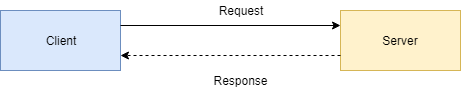
\includegraphics{Img/ClientServerArchitecture}
	\caption{Client Server architecture}
	\label{fig:clientserver}
\end{figure}
Furthermore, the system can be divided into three different subsystems: the presentation layer, the application layer and the data layer as we can see in \autoref{fig:overview}. Additional information are in \autoref{sec:selectedstylesandpatterns}. 
\begin{figure}
	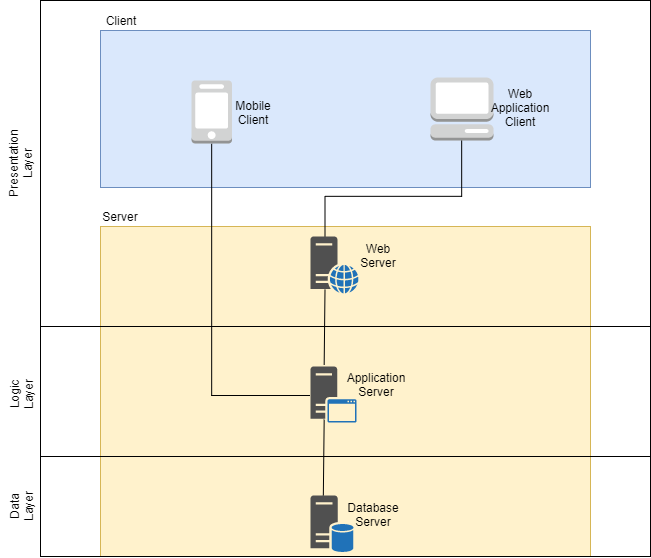
\includegraphics[width=\textwidth, height=\textheight, keepaspectratio=true]{Img/Overview}
	\caption{Overview of the system architecture}
	\label{fig:overview}
\end{figure}





\subsection{Component View}

\subsection{Deployment View}

\subsection{Runtime View}

\subsection{Component Interfaces}

\subsection{Selected architectural styles and patterns}
\label{sec:selectedstylesandpatterns}

\subsection{Other design decision}